\documentclass[12pt]{article}
\usepackage{array}
\usepackage{color}
\usepackage{amsthm}
\usepackage{eufrak}
\usepackage{lipsum}
\usepackage{pifont}
\usepackage{yfonts}
\usepackage{amsmath}
\usepackage{amssymb}
\usepackage{ccfonts}
\usepackage{comment} \usepackage{amsfonts}
\usepackage{fancyhdr}
\usepackage{graphicx}
\usepackage{listings}
\usepackage{mathrsfs}
\usepackage{setspace}
\usepackage{textcomp}
\usepackage{blindtext}
\usepackage{enumerate}
\usepackage{microtype}
\usepackage{xfakebold}
\usepackage{kantlipsum}
%\usepackage{draftwatermark}
\usepackage[spanish]{babel}
\usepackage[margin=1.5cm, top=2cm, bottom=2cm]{geometry}
\usepackage[framemethod=tikz]{mdframed}
\usepackage[colorlinks=true,citecolor=blue,linkcolor=red,urlcolor=magenta]{hyperref}

%//////////////////////////////////////////////////////
% Watermark configuration
%//////////////////////////////////////////////////////
%\SetWatermarkScale{4}
%\SetWatermarkColor{black}
%\SetWatermarkLightness{0.95}
%\SetWatermarkText{\texttt{Watermark}}

%//////////////////////////////////////////////////////
% Frame configuration
%//////////////////////////////////////////////////////
\newmdenv[tikzsetting={draw=gray,fill=white,fill opacity=0},backgroundcolor=none]{Frame}

%//////////////////////////////////////////////////////
% Font style configuration
%//////////////////////////////////////////////////////
\renewcommand{\familydefault}{\ttdefault}
\renewcommand{\rmdefault}{tt}

%//////////////////////////////////////////////////////
% Bold configuration
%//////////////////////////////////////////////////////
\newcommand{\fbseries}{\unskip\setBold\aftergroup\unsetBold\aftergroup\ignorespaces}
\makeatletter
\newcommand{\setBoldness}[1]{\def\fake@bold{#1}}
\makeatother

%//////////////////////////////////////////////////////
% Default font configuration
%//////////////////////////////////////////////////////
\DeclareFontFamily{\encodingdefault}{\ttdefault}{%
  \hyphenchar\font=\defaulthyphenchar
  \fontdimen2\font=0.33333em
  \fontdimen3\font=0.16667em
  \fontdimen4\font=0.11111em
  \fontdimen7\font=0.11111em}



\begin{document}
    %//////////////////////////////////////////////////////
% Heading Configuration
%//////////////////////////////////////////////////////
\pagestyle{fancy}
\thispagestyle{plain}
\fancyhead[RO,L]{\textbf{Teoria de Grafos}}
\fancyhead[LO,L]{\textbf{Tarea 2}}
\setlength{\headheight}{16.0pt}

%//////////////////////////////////////////////////////
% Subsections Configuration
%//////////////////////////////////////////////////////
\renewcommand*\thesubsection{\arabic{subsection}}
\newcounter{counter}
\newlength{\palabra}
\settowidth{\palabra}{counter 999.}
\newcommand{\makeboxlabel}[1]{\fbox{#1.}\hfill}

%//////////////////////////////////////////////////////
% Personalized commands configuration
%//////////////////////////////////////////////////////
\newcommand{\N}{\mathbb{N}}
\newcommand{\Z}{\mathbb{Z}}
\newcommand{\Q}{\mathbb{Q}}
\newcommand{\R}{\mathbb{R}}
\newcommand{\C}{\mathbb{C}}
\newcommand{\re}{\operatorname{Re}}
\newcommand{\im}{\operatorname{Im}}
\newcommand{\Aut}{\operatorname{Aut}}
\newcommand{\GCD}{\operatorname{GCD}}
\newcommand{\LCD}{\operatorname{LCD}}
\linespread{1} %Line spacing

%//////////////////////////////////////////////////////
% Inline code configuration
%//////////////////////////////////////////////////////
\lstset{
gobble=5,
numbers=left,
frame=single,
framerule=1pt,
showtabs=False,
showspaces=False,
showstringspaces=False,
backgroundcolor=\color{gray}}

%//////////////////////////////////////////////////////
% Problem list configuration
%//////////////////////////////////////////////////////
\newenvironment{problems}
  {\begin{list}
     {{\fbseries Problem \arabic{counter}.}}
    {\usecounter{counter}
     \setlength{\labelsep}{1em}
     \setlength{\itemsep}{2pt}
     \setlength{\leftmargin}{2em}
     \setlength{\rightmargin}{0cm}
     \setlength{\itemindent}{1em} }}
{\end{list}}

%//////////////////////////////////////////////////////
% Appendix configuration
%//////////////////////////////////////////////////////
\newenvironment{Appendix}
  {\begin{list}
     {{\fbseries Lemma \arabic{counter}.}}
    {\usecounter{counter}
     \setlength{\labelsep}{1em}
     \setlength{\itemsep}{2pt}
     \setlength{\leftmargin}{2em}
     \setlength{\rightmargin}{0cm}
     \setlength{\itemindent}{1em} }}
{\end{list}}

%//////////////////////////////////////////////////////
% Notes configuration
%//////////////////////////////////////////////////////
\newenvironment{notes}
  {\begin{list}
     {{\fbseries Note \arabic{counter}.}}
    {\usecounter{counter}
     \setlength{\labelsep}{1em}
     \setlength{\itemsep}{2pt}
     \setlength{\leftmargin}{2em}
     \setlength{\rightmargin}{0cm}
     \setlength{\itemindent}{1em} }}
{\end{list}}

%//////////////////////////////////////////////////////
% Activity Information
%//////////////////////////////////////////////////////
\vspace*{-1cm}
\hrule width \hsize \kern 1mm \hrule width \hsize height 2pt
\begin{center}
   \parbox[c]{.32\textwidth}{
   \hspace{1cm}\\
   Sergio Montoya Ramirez\\
   202112171}
%   Luis Ernesto Tejón Rojas\\
%   202113150}
   \hspace*{\fill}
   \parbox[c]{.35\textwidth}{\centering
   Universidad de Los Andes\\
   Tarea 1\\
   Teoria de Grafos\\
   }
   \hspace*{\fill}
   \parbox[c]{.3\textwidth}{
   \begin{flushleft}
      Bogotá D.C., Colombia\\
      \today
   \end{flushleft}}
\end{center}
\hrule width \hsize height 2pt \kern 1mm \hrule width \hsize

\bigskip

\bigskip


    \begin{enumerate}
      \item En este caso el resultado para el hemisferio superior del planeta es:
          \begin{figure}[h]
              \centering
              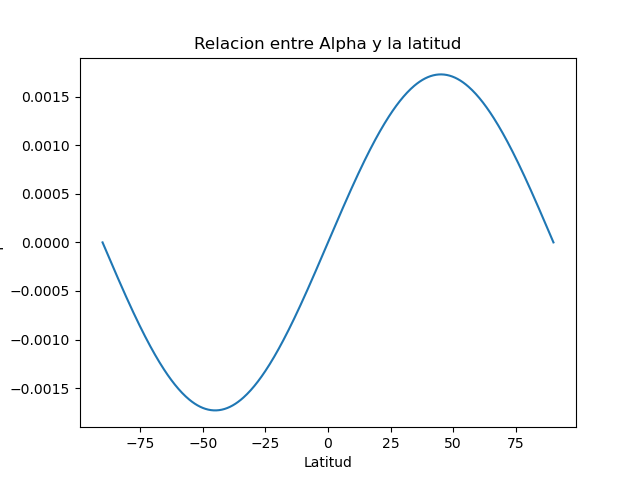
\includegraphics[width=0.8\textwidth]{Graficas/alpha_tierra.png}
              \caption{Grafica de $\alpha$ en función de la latitud.}
              \label{fig:Graficas-alpha_tierra-png}
          \end{figure}
      \item Para este punto creo que lo mejor que podemos hacer es partir desde la ecuación $9.6$ del Taylor la cual es: \[
      \alpha_{max} = \frac{\Omega^2R}{2g_0}
      .\] con esto entonces nos interesa saber que es $g_0$. Para esto utilizaremos la segunda ley de Newton con la fuerza igual a la fuerza gravitatoria e ignorando la centrifuga y centripeta.
      \begin{align*}
        F_G&= mg_0 \\
	G \frac{Mm}{R^2} &= mg_0 \\
	g_0 &= G \frac{M}{R^2} \\
	\alpha_{max} &= \frac{\Omega^2R}{2G \frac{M}{R^2}} \\
	\alpha_{max} &= \frac{\Omega^2R^{3}}{2GM}
      .\end{align*}

    \item Para este punto aprovecharemos el resultado explicitamente anterior pues en tal caso solo nos faltaria averiguar $\Omega$,$R$ y $M$ de cada uno de los planetas para encontrar el resultado de $\alpha_{max}$

      \begin{table}[h]
        \centering
        \caption{Tabla de $\alpha_{max}$ de cada uno de los planetas pedidos.}
        \label{tab:alpha}
        \begin{tabular}{|c|c|c|c|c|}
	  \hline
	  Cuerpo & $\Omega\ \frac{rad}{s}$ & $R\ m$ &  $M\ kg$ & $\alpha_{max}$\\
	  \hline
	  Sol & $\frac{\pi}{1036800}$ & $696.000.000$ & $1.989\times 10^{30}$ & $1.165\times 10^{-5}$ \\
	  Júpiter & $\frac{2\pi}{32400}$ & $71492000$ & $1898\times 10^{24}$ & $0.054$ \\
	Tierra & $7.3\times 10^{-5}$ & $640.000$ & $5.9722\times 10^{24}$ & $0.0017$ \\
	Marte & $\frac{2\pi}{88740}$ & $3396200$ & $0.64\times 10^{24}$ & $0.00228$ \\
	Luna & $\frac{2\pi}{2332800}$ & $1738100$ & $0.073\times 10^{24}$ & $3.90\times 10^{-6}$\\
	\hline
        \end{tabular}
      \end{table}

    \item \textbf{Notas Aclaratorias: }
      \begin{enumerate}
        \item El sol no tiene una velocidad angular exacta dado que es un plasma girando. Esta velocidad varia segun la latitud siendo minima en los polos (Tarda mas o menos 38 dias en dar una vuelta) y maxima en el ecuador (tarda mas o menos 24 dias) por lo tanto esta medida no es exacta como deseariamos pues variaria en cada caso. Aun asi. escogeremos trabajar con la mas rapida para que los efectos se vean mas impresionantes. Con esto entonces tenemos que tarda 24 dias en dar una vuelta por lo  tanto su velocidad es: $\frac{\pi}{12\ days}$. Sin embargo podemos convertir de dias a segundos (para tenerlo en las unidades que nos interesan) y en consecuencia quedaria:
	  \begin{align*}
	    \frac{\pi}{12\ days}\cdot \frac{1\ day}{3600*24} &= \frac{\pi}{1036800}\frac{rad}{s}
	  .\end{align*}
	\item Jupiter se demora aproximadamente $9$ horas en dar una vuelta completa sobre si mismo. Por lo tanto, la velocidad angular de este cuerpo celeste es $\frac{2\pi}{9}\frac{rad}{hrs}$ sin embago dado que necesitamos en $\frac{rad}{s}$ tenemos que hacer la conversión de la siguiente manera:
	  \begin{align*}
          \frac{2\pi}{9\ hrs}\frac{1\ hrs}{3600\ s} = \frac{2\pi}{32400}\frac{rad}{s}
	  .\end{align*}
	\item La tierra se demora $24$ horas en dar una vuelta sobre su eje por lo tanto su $\Omega$ es $\frac{2\pi}{24\ hrs}$ pero lo podemos convertir a $\frac{rad}{s}$ lo que queda como: \[
	\frac{2\pi}{24\ hrs}\frac{1\ hrs}{3600\ s}=\frac{2\pi}{86400}\frac{rad}{s}
	.\] 
      \item Marte se demora $24.65$ horas en dar una vuelta sobre su eje. Por lo tanto su $\Omega$ es $\frac{2\pi}{24.65}$ pero lo podemos convertir a $\frac{rad}{s}$ lo que queda como: \[
      \frac{2\pi}{24.65\ hrs}\frac{1\ hrs}{3600 s}=\frac{2\pi}{88740}\frac{rad}{s}
      .\] 
    \item la luna se demora $27$ dias en dar una vuelta entera sobre su eje. POr lo tanto su $\Omega$ es $\frac{2\pi}{27\ dys}$ pero lo podemos convertir a $\frac{rad}{s}$ lo que queda como: \[
	\frac{2\pi}{27\ dys}\frac{1\ day}{24*3600\ s}=\frac{2\pi}{2332800}\frac{rad}{s}
    .\] 
  \item Los datos utilizados para el punto 3 fueron sacados de una fuente de la nasa en particular estos son los links utilizados:
    \begin{enumerate}
      \item https://nssdc.gsfc.nasa.gov/planetary/factsheet/sunfact.html
      \item https://nssdc.gsfc.nasa.gov/planetary/factsheet/jupiterfact.html
      \item https://nssdc.gsfc.nasa.gov/planetary/factsheet/earthfact.html
      \item https://nssdc.gsfc.nasa.gov/planetary/factsheet/marsfact.html
      \item https://nssdc.gsfc.nasa.gov/planetary/factsheet/moonfact.html
    \end{enumerate}
      \end{enumerate}
    \end{enumerate}
\end{document}
